\section{Foundations}

\subsection{Definitions, identities}
\no Notation
\begin{itemize}
	\item Upper-case letters ($A, B, C, X, Y$): random variables
	\item Lower-case letters ($a, b, c, x, y$): real numbers
	\item $P(X = x) \;=:\; P(x)$
	\item $P(X = x \text{ and } Y = y) \;=:\; P(x, y)$
	\item $P(A = a, \text{ given } B = b) \;=:\; P(a\;|\;b)$
	\item $\int_{\infty}^{+\infty}[\ldots] da \;=:\; \sum_{a\in \mathds{R}} [\ldots] \;=:\; \sum_a[\ldots] $
\end{itemize}
Conditional probability
\begin{itemize}
	\item $P(a\;|\;b) \;=\; \frac{P(a,b)}{P(b)}$
	\item $P(a, b) \;=\; P(a\;|\; b) \;P(b)$
	\item $P(a, b\;|\;c) \;=\;  P(a\;|\;b,c) \; P(b\;|\;c)$
	\item $\sum_a P(a\;|\;b) \;=\; 1$,\quad but \;$\sum_b P(a\;|\;b) \neq 1$, in general
	\item $\sum_b P(a\;|\;b) \; P(b) \;=\; \sum_b P(a,b) \;=\; P(a)$
\end{itemize}
Marginal
\begin{itemize}
	\item $P(a) \;=\; \sum_b P(a\;|\;b) \; P(b)$
\end{itemize}
Bayes theorem
\begin{itemize}
	\item $P(b\;|\;x) \;=\; \frac{1}{P(x)} P(x\;|\;b) \; P(b)$
\vspace{0.5cm}
\end{itemize}
\begin{figure}[h]
	\centering
	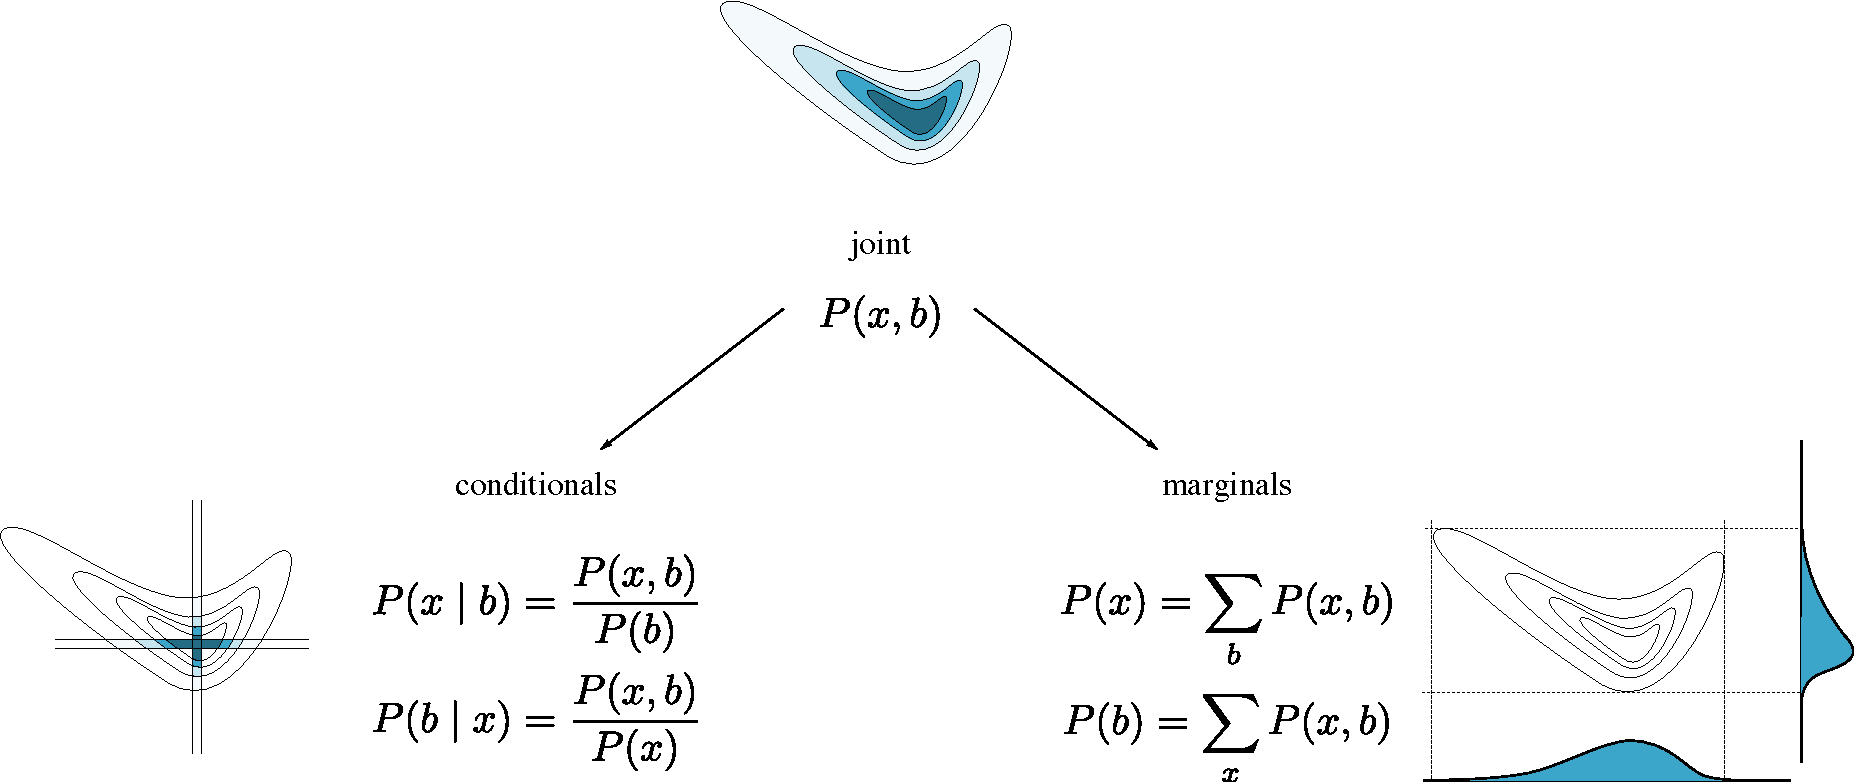
\includegraphics[width=\textwidth]{./figs/Joint-Conditional-Marginal.pdf}
\end{figure}

\subsection{Bayesian inference}
\no Prior, likelihood, posterior
\begin{itemize}
	\item Data: $D = \{x_1, x_2, \ldots x_n\}$, independent measurements.
	\item Model: $M$ with $\theta$: parameter(s) to estimate
	\item Prior: $P(\theta)$
	\item Likelihood: $P(D\;|\;\theta) = P(d_1\;|\;\theta) \;P(d_2\;|\;\theta)\;\ldots \;P(d_n\;|\;\theta) = \prod_{i=1}^n P(d_i\;|\;\theta)$
	\item Unnormalized posterior: $P^\ast(\theta\;|\;D) \;=\; P(D\;|\;\theta) \;P(\theta)$
	\item Normalization: $Z = \sum_\theta P^\ast(\theta\;|\;D)$
	\item Posterior: $P(\theta\;|\;D) = \frac{1}{Z} P^\ast(\theta\;|\;D)$
\end{itemize}
Example

``Three light bulbs of the same make lasted 1, 2 and 5 months of continuous use. Let us estimate the lifetime of this kind of light bulb.''
\begin{itemize}
	\item $D = \{t_1, t_2, t_3\} = \{1,2,5\}$
	\item $M$: Light bulbs have average lifetime of $T$ months.
	\item $P(T) = \frac{1}{1000}$, uniform on [0,1000].
	\item $P(t\;|\;T) = \frac{1}{T}\exp\left(-\frac{t}{T}\right)$
	\item $P(D\;|\;T) = \prod_i P(t_i\;|\; T) = \prod_{i=1}^3 \frac{1}{T}\exp\left(-\frac{t_i}{T}\right) = \frac{1}{T^3} \exp\left(-\frac{1 + 2 + 5}{T}\right)$
	\item $P^\ast(T\;|\;D) = \frac{1}{T^3} \exp\left(-\frac{8}{T}\right)$
	\item $Z$ and  $P(T\;|\;D)$ can be determined numerically:
\begin{lstlisting}[language=python]
import numpy as np

T_arr = np.linspace(0.1, 1000, 10_000)
Pstar_arr = 1.0/T_arr**3 * np.exp(-8/T_arr)
Z = np.sum(Pstar_arr)
P_arr = Pstar_arr / Z
\end{lstlisting}
	yielding $Z = 0.1562$
	\item $\mathbb{E}(T\;|\;D) = \sum_T T \;P(T\;|\;D)$ 
	\item $\text{std}(T\;|\;D) = \sqrt{\sum_T (T - \mathbb{E}(T))^2 \; P(T\;|\;D)}$
\begin{lstlisting}[language=python]
T_ev = np.sum(T_arr * P_arr)
T_std = np.sqrt(np.sum((T_arr - T_ev)**2 * P_arr))
\end{lstlisting}
	yielding $\mathbb{E}(T\;|\;D) = 7.937$, \quad $\text{std}(T\;|\;D) = 14.48$.
\end{itemize}


\subsection{Model comparison}
\no New definition: Evidence
\begin{itemize}
	\item Data: $D$
	\item Model 1: $M_1$ with parameter $\theta_1$ and prior $P(\theta_1\;|\; M_1)$, and likelihood $P(D\;|\;\theta_1, M_1)$
	\item Model 2: $M_2$ with parameter $\theta_2$ and prior $P(\theta_2\;|\; M_2)$, and likelihood $P(D\;|\;\theta_2, M_2)$
	\item Prior on models: $P(M_1) = 0.5$, \; $P(M_2) = 0.5$.
	\item Evidence for each model: $P(D\;|\;M_i) = \sum_\theta P(D\;|\;\theta_i, M_i) P(\theta_i\;|\;M_i)$
	\item Unnormalized posterior: $P^\ast(M_1\;|\;D) = P(D\;|\;M_1) \; P(M_1)$,\quad and $P^\ast(M_2\;|\;D) = P(D\;|\;M_2) \; P(M_2)$
	\item Normalization: $Z = P^\ast(M_1\;|\;D) + P^\ast(M_2\;|\;D)$.
\end{itemize}
Example

``Waiting for my baggage at the airport carousel, there are two possibilities: 1) It could miss the plane, and will never come, or 2) It was on the plane and it had a 1/20 chance of arriving within any of the 1-minute intervals between 0 and 20 minutes. Now, given what is the posterior probability of model 2 given that 14 minutes has passed and the bas has not arrived?''
\begin{itemize}
	\item $D = \{\text{Bag has not arrived after } t_\text{wait}=14 \text{ minutes}\}$
	\item $M_1$: It never arrives, $P(D\;|\;M_1) = 1$
	\item $M_2$: It shows up some time between 0 and 20 minutes, $P(t_\text{bag}\;|\;M_2) = 1/20$ for $t_\text{bag} \in [0, 20]$, and the likelihood is $P(D\;|\;t_\text{bag}, M_2) = 1$, if $t_\text{bag} > t_\text{wait}$, and 0 otherwise.
	\item $P(M_1) = 0.1$, \quad $P(M_2)= 0.9$
	\item $P(D\;|\;M_1)$ = 1
	\item $P(D\;|\;M_2) = \sum_{t_\text{bag}} P(D\;|\;t_\text{bag}, M_2) \;P(t_\text{bag}\;|\;M_2) = \sum_{t_\text{bag}} [t_\text{bag} > 14] \times\frac{1}{20} = \frac{20 - 14}{20}$
	\item $P^\ast(M_1\;|\;D) = 1 \times 0.1$, \quad $P^\ast(M_2\;|\;D) = \frac{20 - 14}{20}\times 0.9$
	\item $Z = 0.1 + \frac{3}{10}\times 0.9 = 0.37$
	\item $P(M_2\;|\;D) = P^\ast(M_2\;|\;D) / Z = 0.7297$.
\end{itemize}
We can also plot $P(M_2\;|\;t_\text{wait})$ for all waiting times between 0 and 20 minutes.
\begin{figure}[h]
	\centering
	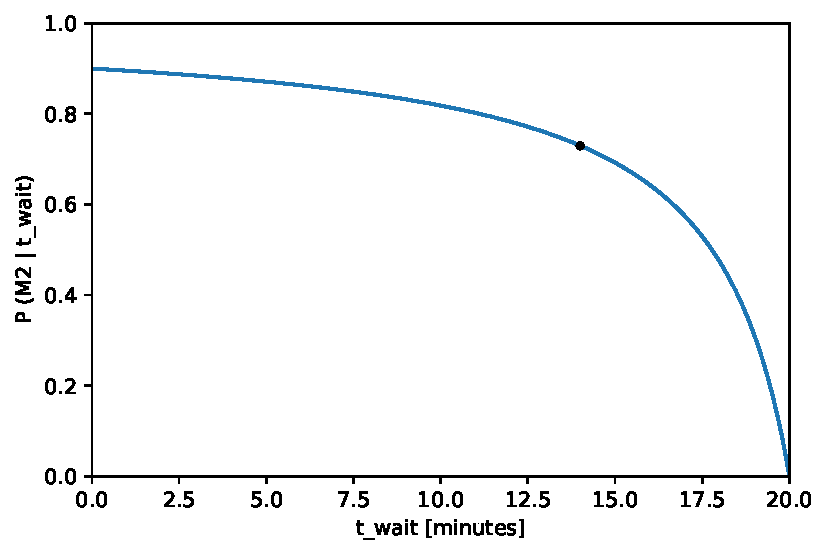
\includegraphics[width=0.5\textwidth]{figs/Baggage_wait.pdf}
\end{figure}


\subsection{Prediction}
\no New definition: Predictive distribution
\begin{itemize}
	\item Data: $D = \{x_1, x_2, \ldots x_n\}$
	\item Model: $M$ with parameter $\theta$, prior $P(\theta)$ and likelihood $P(x\;|\;\theta)$
	\item Posterior: $P(\theta\;|\;D) = P^\ast(\theta\;|\;D) / Z = \ldots$ (see previous sections)
	\item Predictive distribution: $P(X_{n+1} = x\;|\;D) = \sum_\theta P(x\;|\theta)\; P(\theta\;|\;D)$
	\item Customized prediction: $P(f(\theta)\;|\;D) = \sum_\theta f(\theta)\; P(\theta\;|\;D)$
\end{itemize}
Example

``Two player, A and B are playing a game of luck, where at the beginning of the game a ball is rolled on a pool table to divide the table in two un-equal halves: A's side and B's side. In each subsequent round, a ball is rolled. A point is given to the player on whose side the ball stops. A and B are playing this game until one of them reaches 6 points. The current score is 5 to 3 in favor of A. What is the chance that A will win this game?''
\begin{itemize}
	\item $D = \{n_A = 5, n_B = 3\}$
	\item $M$, first ball: $P(b) = 1$ in $[0,1]$
	\item $P(\text{A scores}\;|\;b) = b$
	\item $P(D\;|\;b) = \text{Binomial}(5\;|\;5 + 3, \;b)$
	\item $P^\ast(b_0\;|\;D) = \text{Binomial}(5\;|\; 8, b) \times 1$
	\item $Z = \sum_{b} \text{Binomial}(5\;|\; 8, b)$ can be calculated numerically
\begin{lstlisting}[language=python]
import numpy as np
from scipy.stats import binom

b_arr = np.linspace(0, 1, 1000)
Pstar_arr = binom.pmf(5, 8, b_arr)
Z = np.sum(Pstar_arr)
\end{lstlisting}
	\item $P(\text{A wins}\;|\;b, D) = 1 - P(\text{B wins}\;|\;b, D) = 1 - (1 - b)^3 = f(b)$
	\item $P(\text{A wins}\;|\;D) = \sum_{b} f(b) P^\ast(b\;|\;D) / Z$
\begin{lstlisting}[language=python]
P_arr = Pstar_arr / Z
P_Awins = np.sum((1 - (1 - b_arr)**3) * P_arr)
\end{lstlisting}
	yielding $P(\text{A wins}\;|\;D) = 0.909$
\end{itemize}





